\documentclass[11pt,a4paper]{article}

% ── Packages ──
\usepackage[utf8]{inputenc}
\usepackage[T1]{fontenc}
\usepackage{amsmath,amssymb}
\usepackage{physics}
\usepackage{siunitx}
\usepackage{booktabs}
\usepackage{geometry}
\usepackage{hyperref}
\usepackage{enumitem}
\usepackage{float}
\usepackage{graphicx}

\geometry{margin=2.5cm}
\hypersetup{colorlinks=true,linkcolor=blue,citecolor=blue,urlcolor=blue}

\title{Residual Gas Velocity Above a Stopped Propeller Blade\\
       in Dense Xenon: A Mechanism-by-Mechanism Analysis}
\author{}
\date{}

\begin{document}
\maketitle

% ══════════════════════════════════════════════════════════════════════════════
% PART I: THEORY
% ══════════════════════════════════════════════════════════════════════════════

\part*{Part I: Theory}

% ══════════════════════════════════════════════════════════════════════════════
\section{Problem Definition}
\label{sec:problem}
% ══════════════════════════════════════════════════════════════════════════════

A horizontal propeller with $n$ equally-spaced blades (NACA\,0012 airfoil
cross-section) rotates inside a vertical cylindrical vessel filled with xenon
gas at high pressure. The propeller sweeps through a prescribed angle
$\theta = 2\pi/n$ in a time $t_\mathrm{rot}$, starting from rest and returning
to rest via a bang-bang motion profile. We seek the residual gas velocity at a
height $z_\mathrm{obs}$ above the upper blade surface, evaluated at a time
$t_\mathrm{obs}$ after the blade has stopped.

Two configurations are analysed:
\begin{itemize}[nosep]
  \item \textbf{2-arm propeller}: $n = 2$, sweep angle $\theta = \pi$ (180°)
  \item \textbf{8-arm propeller}: $n = 8$, sweep angle $\theta = \pi/4$ (45°)
\end{itemize}

\subsection{Parameters}

\begin{table}[H]
\centering
\caption{Variable parameters (with default values).}
\label{tab:params}
\begin{tabular}{llll}
\toprule
Symbol & Description & Default & Units \\
\midrule
$n$                   & Number of blade arms            & 2 or 8 & --- \\
$c$                   & Blade chord length              & 0.16  & m   \\
$\theta$              & Sweep angle ($= 2\pi/n$)        & ---   & rad \\
$m_\mathrm{blade}$   & Mass of each blade              & 0.25  & kg  \\
$m_\mathrm{plate}$   & Mass of each carrier plate      & 0.25  & kg \\
$\tau$               & Motor torque                     & 60    & N$\cdot$m \\
$z_\mathrm{obs}$     & Observation height above blade top & 0.005 & m \\
$t_\mathrm{obs}$     & Observation time after stop      & 0.5   & s   \\
\midrule
\multicolumn{4}{l}{\textit{Carrier plate parameters (Phase 2)}} \\
$m_\mathrm{carrier}$ & Carrier plate mass               & 0.25  & kg  \\
$r_0$                & Initial radial position          & 0.8   & m   \\
$F_\mathrm{act}$     & Linear actuator force            & 20    & N   \\
$C_d^\mathrm{carrier}$ & Carrier drag coefficient       & 0.1   & --- \\
\bottomrule
\end{tabular}
\end{table}

\begin{table}[H]
\centering
\caption{Fixed parameters.}
\label{tab:fixed}
\begin{tabular}{lll}
\toprule
Parameter & Value & Description \\
\midrule
$R$            & \SI{1.6}{m}        & Blade span (hub to tip) \\
$P$            & \SI{15}{bar}       & Xenon pressure \\
$T$            & \SI{300}{K}        & Gas temperature \\
NACA profile   & 0012               & Symmetric, 12\% thickness \\
$\alpha$       & $0^\circ$          & Angle of attack \\
$\Delta D$     & \SI{0.01}{m}       & Vessel inner diameter surplus over propeller \\
\bottomrule
\end{tabular}
\end{table}

\subsection{Geometry and Coordinate System}

The blade rotates in the $xy$-plane. The $z$-axis points upward from
the blade centre-plane. The NACA\,0012 blade has maximum thickness
$t_\mathrm{max} = 0.12\,c$, so the upper blade surface is at
$z_\mathrm{blade} = t_\mathrm{max}/2 = 0.06\,c$ above the rotation
axis. The cylindrical vessel has inner radius
\begin{equation}
  R_\mathrm{cyl} = R + \frac{\Delta D}{2}\,.
\end{equation}
The tip clearance is $\Delta r = \Delta D / 2$.


% ══════════════════════════════════════════════════════════════════════════════
\section{Xenon Gas Properties}
\label{sec:gas}
% ══════════════════════════════════════════════════════════════════════════════

Xenon is a monatomic ideal gas to good approximation at \SI{15}{bar},
\SI{300}{K} (compressibility factor $Z \approx 0.98$).

\paragraph{Density.}
\begin{equation}
  \rho = \frac{P M_\mathrm{Xe}}{R_g T}\,,
  \label{eq:density}
\end{equation}
where $M_\mathrm{Xe} = \SI{0.13129}{kg/mol}$ and
$R_g = \SI{8.314}{J/(mol\cdot K)}$.

\paragraph{Dynamic viscosity.}
The viscosity of Xe is nearly pressure-independent at moderate densities.
At $T = \SI{300}{K}$:
\begin{equation}
  \mu \approx \SI{2.32e-5}{Pa\cdot s}\,.
\end{equation}

\paragraph{Kinematic viscosity.}
\begin{equation}
  \nu = \frac{\mu}{\rho}\,.
  \label{eq:nu}
\end{equation}

\paragraph{Speed of sound.}
For a monatomic ideal gas with $\gamma = 5/3$:
\begin{equation}
  c_s = \sqrt{\frac{\gamma R_g T}{M_\mathrm{Xe}}}\,.
  \label{eq:cs}
\end{equation}


% ══════════════════════════════════════════════════════════════════════════════
\section{Blade Kinematics: Bang-Bang Motion Profile}
\label{sec:kinematics}
% ══════════════════════════════════════════════════════════════════════════════

The propeller executes a \emph{bang-bang} motion profile: it accelerates
under constant motor torque $\tau$, then decelerates under reversed
torque $-\tau$. The equation of motion is:
\begin{equation}
  I\,\frac{d\omega}{dt} = \pm\tau\,,
  \label{eq:EOM}
\end{equation}
where the upper sign applies during acceleration and the lower during
deceleration.

\paragraph{Moment of Inertia.}
The system consists of $n$ blades (uniform rods of mass $m_\mathrm{blade}$
extending from $r = 0$ to $r = R$) and $n$ carrier plates (point masses
$m_\mathrm{plate}$ at initial radial position $r_0 = R/2$):
\begin{equation}
  I = n \times \frac{1}{3}\,m_\mathrm{blade}\,R^2
    + n \times m_\mathrm{plate}\,r_0^2\,.
  \label{eq:I}
\end{equation}

\paragraph{Closed-Form Solution (No Aerodynamic Drag).}
For the symmetric bang-bang profile, the switching occurs at $\theta/2$:
\begin{align}
  \alpha &= \frac{\tau}{I}\,,
    \label{eq:alpha} \\
  t_\mathrm{rot} &= 2\sqrt{\frac{\theta\, I}{\tau}}\,,
    \label{eq:trot} \\
  \omega_\mathrm{max} &= \sqrt{\frac{\theta\,\tau}{I}}\,.
    \label{eq:omega_max}
\end{align}

\paragraph{Peak Tip Velocity.}
\begin{equation}
  V_\mathrm{tip} = \omega_\mathrm{max}\,R\,.
  \label{eq:Vtip}
\end{equation}


% ══════════════════════════════════════════════════════════════════════════════
\section{Flow Regime}
\label{sec:regime}
% ══════════════════════════════════════════════════════════════════════════════

\paragraph{Mach Number.}
The tip Mach number is
\begin{equation}
  \mathrm{Ma}_\mathrm{tip}
    = \frac{V_\mathrm{tip}}{c_s}\,.
  \label{eq:Mach}
\end{equation}
For $\mathrm{Ma} < 0.3$, the flow is \emph{incompressible}: density
variations are negligible ($< 5\%$), and the continuity equation
simplifies to $\nabla \cdot \mathbf{v} = 0$.

\paragraph{Reynolds Number.}
The chord-based Reynolds number at the tip is
\begin{equation}
  \mathrm{Re}_c = \frac{V_\mathrm{tip}\,c}{\nu}\,.
  \label{eq:Re}
\end{equation}
For $\mathrm{Re}_c > 5 \times 10^5$, the boundary layer is
\emph{fully turbulent}.


% ══════════════════════════════════════════════════════════════════════════════
\section{Boundary Layer on the Upper Surface}
\label{sec:BL}
% ══════════════════════════════════════════════════════════════════════════════

Since we are interested in the flow \emph{above} the blade, only the
upper-surface boundary layer (BL) matters.

\paragraph{Turbulent BL Thickness.}
For a turbulent BL developing from the leading edge over a flat plate
of length $c$ at Reynolds number $\mathrm{Re}_c$, the standard
$\tfrac{1}{7}$-power-law result gives:
\begin{align}
  \delta &= 0.37\,c\;\mathrm{Re}_c^{-1/5}\,,
    \label{eq:delta} \\
  \theta_\mathrm{BL} &= \frac{7}{72}\,\delta\,,
    \label{eq:theta_BL} \\
  \delta^* &= \frac{1}{8}\,\delta\,,
    \label{eq:dstar}
\end{align}
where $\delta$ is the BL thickness, $\theta_\mathrm{BL}$ the momentum
thickness, and $\delta^*$ the displacement thickness.

\paragraph{Skin Friction and Friction Velocity.}
\begin{align}
  C_f &= 0.0592\;\mathrm{Re}_c^{-1/5}\,,
    \label{eq:Cf} \\
  u_\tau &= V_\mathrm{tip}\,\sqrt{\frac{C_f}{2}}\,.
    \label{eq:utau}
\end{align}

\paragraph{Vertical Geometry.}
The upper blade surface sits at $z_\mathrm{blade} = 0.06\,c$ above the
rotation axis. The BL extends to
\begin{equation}
  z_\mathrm{BL} = z_\mathrm{blade} + \delta\,.
\end{equation}
The gap between the top of the BL and the observation height is
\begin{equation}
  \Delta z_\mathrm{gap} = z_\mathrm{obs} - \delta\,.
  \label{eq:gap}
\end{equation}

\paragraph{Initial Velocity Profile in the Lab Frame.}
In the blade's reference frame, the BL velocity follows a
$\tfrac{1}{7}$-power law. Transforming to the lab frame (where the gas
is initially at rest and the blade moves at $V$):
\begin{equation}
  u_\mathrm{lab}(z) =
  \begin{cases}
    V\bigl[1 - (z/\delta)^{1/7}\bigr] & 0 < z \le \delta \\
    0 & z > \delta
  \end{cases}
  \label{eq:ulab}
\end{equation}


% ══════════════════════════════════════════════════════════════════════════════
\section{Mechanism 1: Turbulent Eddy Diffusion}
\label{sec:eddies}
% ══════════════════════════════════════════════════════════════════════════════

After the blade stops, the momentum in the BL (equation~\ref{eq:ulab})
can diffuse vertically into the quiescent gas above. The evolution is
governed by the one-dimensional diffusion equation:
\begin{equation}
  \frac{\partial u}{\partial t}
  = \frac{\partial}{\partial z}
    \left[\nu_\mathrm{eff}(z,t)\,\frac{\partial u}{\partial z}\right],
  \label{eq:diffusion}
\end{equation}
with boundary conditions $u(0,t) = 0$ (no-slip on stationary blade) and
$u(z \to \infty, t) = 0$.

\paragraph{Turbulent Viscosity Profile.}
The effective viscosity is $\nu_\mathrm{eff} = \nu + \nu_t(z,t)$.
At $t = 0$, the turbulent viscosity follows the two-layer model:
\begin{equation}
  \nu_t(z, 0) =
  \begin{cases}
    \kappa\, u_\tau\, z & z < 0.2\,\delta \\
    0.018\, V\, \delta^* & 0.2\,\delta \le z < \delta \\
    0 & z \ge \delta
  \end{cases}
  \label{eq:nut_profile}
\end{equation}
where $\kappa = 0.41$ is the von K\'arm\'an constant.

\paragraph{Turbulence Decay.}
Once the blade stops, there is no energy input to sustain the
turbulence. The eddies decay on the large-eddy turnover timescale:
\begin{equation}
  t_e = \frac{\delta}{u'}\,,
  \label{eq:teddy}
\end{equation}
where $u' \approx 0.05\,V$ is the outer-layer turbulence intensity.
We model the decay as exponential with an $e$-folding time of $2\,t_e$:
\begin{equation}
  \nu_t(z,t) = \nu_t(z,0)\;\exp\!\left(-\frac{t}{2\,t_e}\right).
  \label{eq:nut_decay}
\end{equation}

\paragraph{Diffusion Length Scales.}
Turbulent diffusion reach during the decay period:
\begin{equation}
  \ell_\mathrm{turb} \sim \sqrt{\nu_t^\mathrm{outer} \times 2\,t_e}\,.
  \label{eq:ell_turb}
\end{equation}
Molecular diffusion reach over $t_\mathrm{obs}$:
\begin{equation}
  \ell_\mathrm{mol} = \sqrt{\nu\, t_\mathrm{obs}}\,.
  \label{eq:ell_mol}
\end{equation}
Maximum reach from BL top:
\begin{equation}
  z_\mathrm{max} = \delta + \ell_\mathrm{turb} + \ell_\mathrm{mol}\,.
\end{equation}

\paragraph{Result.}
If $z_\mathrm{max} < z_\mathrm{obs}$, momentum cannot reach the
observation point:
\begin{equation}
  \boxed{u(z_\mathrm{obs},\, t_\mathrm{obs}) = 0
    \quad \text{(eddy diffusion)}}
\end{equation}


% ══════════════════════════════════════════════════════════════════════════════
\section{Mechanism 2: Bulk Swirl and Angular Momentum}
\label{sec:swirl}
% ══════════════════════════════════════════════════════════════════════════════

\paragraph{Angular Impulse.}
The drag on all $n$ blades deposits tangential momentum into the gas.
The drag torque:
\begin{equation}
  \tau_\mathrm{drag} = n \int_0^R r\, \tfrac{1}{2}\rho\,[\omega r]^2\,c\,C_d\, dr
      = \frac{n\,\rho\,\omega^2\,c\,C_d\,R^4}{8}\,.
  \label{eq:torque}
\end{equation}

\paragraph{Momentum Confinement.}
The angular momentum is deposited \emph{exclusively} within the
boundary layers on the blade surfaces. The time for momentum to diffuse
across the gap by molecular viscosity:
\begin{equation}
  t_\mathrm{visc}
    = \frac{(\Delta z_\mathrm{gap})^2}{\nu}\,.
  \label{eq:tvisc}
\end{equation}

\paragraph{Ekman Pumping.}
In a rotating fluid adjacent to a boundary, the Ekman layer drives a
secondary circulation:
\begin{equation}
  \delta_E = \sqrt{\frac{\nu_\mathrm{eff}}{\Omega}}\,,
  \qquad
  w_E = \sqrt{\nu_\mathrm{eff}\,\Omega}\,.
  \label{eq:Ekman}
\end{equation}

\paragraph{Ekman Spin-Up Time.}
\begin{equation}
  t_\mathrm{Ekman} = \frac{H}{\sqrt{\nu_\mathrm{eff}\,\Omega}}\,.
  \label{eq:tEkman}
\end{equation}

\paragraph{Result.}
If $t_\mathrm{visc} \gg t_\mathrm{obs}$ and $t_\mathrm{Ekman} \gg t_\mathrm{obs}$:
\begin{equation}
  \boxed{u(z_\mathrm{obs},\, t_\mathrm{obs}) \approx 0
    \quad \text{(bulk swirl)}}
\end{equation}


% ══════════════════════════════════════════════════════════════════════════════
\section{Mechanism 3: Displacement (Potential) Flow}
\label{sec:potential}
% ══════════════════════════════════════════════════════════════════════════════

The NACA\,0012 blade has finite thickness $t_\mathrm{max} = 0.12\,c$. As
it moves through the gas, it displaces fluid. The displacement velocity
at height $z$:
\begin{equation}
  w_\mathrm{disp}(z)
    \sim V \,\frac{(t_\mathrm{max}/2)^2}{z^2 + (t_\mathrm{max}/2)^2}\,.
  \label{eq:wdisp}
\end{equation}

\paragraph{Acoustic Clearing Time.}
When the blade stops, the potential flow field propagates away at the
speed of sound:
\begin{equation}
  t_\mathrm{acoustic} = \frac{R}{c_s}\,.
  \label{eq:tacoustic}
\end{equation}

\paragraph{Result.}
For $t_\mathrm{obs} \gg t_\mathrm{acoustic}$:
\begin{equation}
  \boxed{u(z_\mathrm{obs},\, t_\mathrm{obs}) = 0
    \quad \text{(potential flow)}}
\end{equation}


% ══════════════════════════════════════════════════════════════════════════════
\section{Mechanism 4: Pressure Pulse from Deceleration}
\label{sec:pressure}
% ══════════════════════════════════════════════════════════════════════════════

When the blade decelerates to rest, the change in momentum creates a
pressure transient.

\paragraph{Amplitude.}
The pressure perturbation:
\begin{equation}
  \Delta p \sim \rho\, V_\mathrm{tip}^2\,.
  \label{eq:dp}
\end{equation}
The induced acoustic velocity:
\begin{equation}
  \Delta u \sim \frac{\Delta p}{\rho\, c_s}
            = \frac{V_\mathrm{tip}^2}{c_s}\,.
  \label{eq:du_acoustic}
\end{equation}

\paragraph{Result.}
The pulse is transient and passes through $z_\mathrm{obs}$:
\begin{equation}
  \boxed{u(z_\mathrm{obs},\, t_\mathrm{obs}) = 0
    \quad \text{(pressure pulse)}}
\end{equation}


% ══════════════════════════════════════════════════════════════════════════════
\section{Mechanism 5: Secondary Flows}
\label{sec:secondary}
% ══════════════════════════════════════════════════════════════════════════════

\paragraph{Tip Clearance Flow.}
For NACA\,0012 at $\alpha = 0$: there is \emph{no lift}, hence
\emph{no pressure difference} across the blade:
\begin{equation}
  \Delta p_\mathrm{tip} = 0 \qquad (\alpha = 0)\,.
\end{equation}

\paragraph{Centrifugal Effects.}
The tangential wake gas experiences centrifugal acceleration:
\begin{equation}
  a_\mathrm{cent} = \frac{V_\mathrm{tip}^2}{R}\,.
  \label{eq:acent}
\end{equation}
The wake is \emph{tangential}: it flows \emph{along} the cylindrical
wall, not \emph{into} it. There is no face-on impingement to deflect
flow into the axial direction.

\paragraph{Result.}
\begin{equation}
  \boxed{u(z_\mathrm{obs},\, t_\mathrm{obs}) = 0
    \quad \text{(secondary flows)}}
\end{equation}


% ══════════════════════════════════════════════════════════════════════════════
\section{Mechanism 6: Vortex Shedding}
\label{sec:vortex}
% ══════════════════════════════════════════════════════════════════════════════

For a \emph{non-lifting} blade ($\alpha = 0$), there is no net
circulation, hence no macroscopic starting/stopping vortex.

The Strouhal number for drag-induced shedding:
\begin{equation}
  \mathrm{St} = \frac{f\, t_\mathrm{max}}{V} \approx 0.21\,.
\end{equation}
But NACA\,0012 at $\alpha = 0$ is streamlined: coherent vortex shedding
is strongly suppressed. Any residual shed vortices are confined to the
blade plane (within $\sim\delta$ of the surface).

\begin{equation}
  \boxed{u(z_\mathrm{obs},\, t_\mathrm{obs}) = 0
    \quad \text{(vortex shedding)}}
\end{equation}


% ══════════════════════════════════════════════════════════════════════════════
\section{Vessel Confinement Effects}
\label{sec:confinement}
% ══════════════════════════════════════════════════════════════════════════════

The propeller operates inside a cylindrical pressure vessel of height
$H$ and inner radius $R_\mathrm{cyl} = R + \Delta r$.

\paragraph{Wall Boundary Layers.}
The Stokes penetration depth during the sweep:
\begin{equation}
  \delta_\mathrm{wall} \sim \sqrt{\nu\, t_\mathrm{rot}}\,.
\end{equation}

\paragraph{Tip-Gap Couette Flow.}
The tip-gap Reynolds number:
\begin{equation}
  \mathrm{Re}_\mathrm{gap} = \frac{V_\mathrm{tip}\,\Delta r}{\nu}\,.
\end{equation}
This Couette-like flow is purely \emph{tangential} with no axial component.

\paragraph{Reflected Pressure Waves.}
The reverberation time:
\begin{equation}
  t_\mathrm{reverb} = \frac{\sqrt{(2R_\mathrm{cyl})^2 + H^2}}{c_s}\,.
\end{equation}
These waves induce oscillatory velocities but leave no persistent flow.

\paragraph{Result.}
No confinement effect introduces a new vertical transport mechanism.
All wall-related phenomena are either tangential, too slow, or transient.


% ══════════════════════════════════════════════════════════════════════════════
\section{Phase 2: Carrier Radial Slide}
\label{sec:carrier}
% ══════════════════════════════════════════════════════════════════════════════

After the blade rotation completes (Phase 1), the carrier plate slides
radially along the blade arm (Phase 2). The motions are \emph{sequential,
not simultaneous}, to avoid Coriolis torque coupling and time-varying
moment of inertia.

\paragraph{Carrier Geometry.}
The carrier plate is a rectangular box:
\begin{itemize}[nosep]
  \item Surface area: $160 \times 160\,\mathrm{mm}^2$
  \item Height: $h_c = \SI{5}{mm}$
  \item All edges: symmetric sharp leading edges (wedge profile, half-angle $\sim 10^\circ$)
  \item Frontal area: $A_f = w_c \times h_c = \SI{0.16}{m} \times \SI{0.005}{m} = \SI{8e-4}{m^2}$
\end{itemize}

\paragraph{Bang-Bang Linear Motion.}
The carrier executes a bang-bang linear motion with constant actuator
force $F_\mathrm{act}$:
\begin{equation}
  m_\mathrm{carrier}\,\frac{d^2 x}{dt^2} = \pm F_\mathrm{act}\,.
\end{equation}
The closed-form solution (neglecting drag):
\begin{align}
  a &= \frac{F_\mathrm{act}}{m_\mathrm{carrier}}\,,
    \label{eq:a_carrier} \\
  t_\mathrm{slide} &= 2\sqrt{\frac{\Delta r\, m_\mathrm{carrier}}{F_\mathrm{act}}}\,,
    \label{eq:tslide} \\
  V_\mathrm{max} &= \sqrt{\frac{\Delta r\, F_\mathrm{act}}{m_\mathrm{carrier}}}\,.
    \label{eq:Vmax_carrier}
\end{align}
where $\Delta r = r_0$ for worst-case travel from initial position to center.

\paragraph{Carrier Boundary Layer.}
The carrier plate develops its own boundary layer as it slides through
the gas:
\begin{equation}
  \delta_c = 0.37\,L_c\,\mathrm{Re}_L^{-1/5}\,,
\end{equation}
where $L_c = \SI{0.16}{m}$ is the carrier width and
$\mathrm{Re}_L = V_\mathrm{max}\,L_c/\nu$.

\paragraph{Eddy Diffusion After Slide Stops.}
The same analysis as for the blade applies: momentum in the carrier BL
diffuses upward with decaying turbulent viscosity. The maximum reach is:
\begin{equation}
  z_\mathrm{max}^c = \delta_c + \ell_\mathrm{turb}^c + \ell_\mathrm{mol}\,.
\end{equation}

\paragraph{Result.}
If $z_\mathrm{max}^c < z_\mathrm{obs}$, the carrier slide contributes
zero residual velocity at the observation point:
\begin{equation}
  \boxed{u(z_\mathrm{obs},\, t_\mathrm{obs}) = 0
    \quad \text{(carrier slide)}}
\end{equation}


% ══════════════════════════════════════════════════════════════════════════════
\section{Phase 3: Vertical Plate Lift}
\label{sec:lift}
% ══════════════════════════════════════════════════════════════════════════════

After both blade rotation (Phase 1) and carrier slide (Phase 2) complete,
the carrier plate is lifted vertically to a height $z_\mathrm{lift}$ above
its original position. This vertical motion creates a new boundary layer
(Stokes layer) that must settle before measurements can begin.

\paragraph{Lift Parameters.}
\begin{table}[H]
\centering
\caption{Phase 3 parameters (vertical lift).}
\label{tab:lift_params}
\begin{tabular}{llll}
\toprule
Symbol & Description & Default & Units \\
\midrule
$z_\mathrm{lift}$ & Lift height & 5 & mm \\
$t_\mathrm{lift}$ & Lift duration & 1.0 & s \\
$t_\mathrm{wait}$ & Wait time after lift & 0.5 & s \\
$u_c$ & Quiescence cutoff velocity & 0.1 & mm/s \\
\bottomrule
\end{tabular}
\end{table}

\paragraph{Bang-Bang Vertical Motion.}
The plate executes a bang-bang vertical motion:
\begin{align}
  a_\mathrm{lift} &= \frac{4\,z_\mathrm{lift}}{t_\mathrm{lift}^2}\,,
    \label{eq:alift} \\
  V_\mathrm{lift} &= \frac{2\,z_\mathrm{lift}}{t_\mathrm{lift}}\,.
    \label{eq:Vlift}
\end{align}

\paragraph{Stokes Layer.}
The impulsively started vertical motion creates a Stokes layer with
thickness:
\begin{equation}
  \delta_\mathrm{Stokes} = \sqrt{\nu\, t_\mathrm{lift}}\,.
  \label{eq:delta_stokes}
\end{equation}

\paragraph{Three Velocity Profiles.}
After Phase 3, we evaluate three distinct velocity profiles:

\textbf{Profile 1} (blade BL diffusion): The original blade boundary
layer from Phase 1, evaluated at time $t = t_\mathrm{slide} + t_\mathrm{lift}
+ t_\mathrm{wait}$ after the blade rotation stopped. This profile uses the
same diffusion model as Section~\ref{sec:eddies}, but at a much longer
evaluation time. Due to the short turbulence decay time ($\sim$3--18 ms)
compared to the evaluation time ($\sim$1.7 s), this profile is typically
fully decayed.

\textbf{Profile 2} (carrier slide BL diffusion): The boundary layer from
the carrier slide (Phase 2), evaluated at time $t = t_\mathrm{lift} +
t_\mathrm{wait}$ after the slide stopped. This uses the same diffusion
model as Profile 1, with parameters from the carrier boundary layer.

\textbf{Profile 3} (Stokes layer from lift): The boundary layer created
by the vertical lift, evaluated at time $t_\mathrm{wait}$ after the lift
stops. The solution is the classical Stokes first problem (impulsively
stopped plate):
\begin{equation}
  u(z, t) = V_\mathrm{lift}\,\mathrm{erfc}\!\left(\frac{z - z_\mathrm{lift}}{2\sqrt{\nu_\mathrm{eff}\,t}}\right),
  \label{eq:stokes_erfc}
\end{equation}
where $\nu_\mathrm{eff}$ accounts for the initial Stokes layer thickness.
The coordinate system is RF1 (reference frame 1), where $z = 0$
is the original blade/carrier surface, and the lifted plate is now at
$z = z_\mathrm{lift}$.

\paragraph{Quiescence Height.}
For each profile, we find the \emph{quiescence height} $z_q$: the height
at which the velocity drops below the cutoff $u_c$:
\begin{equation}
  z_q = \min\{z : u(z) < u_c\}\,.
  \label{eq:zq}
\end{equation}
For Profile 3, we search for $z_q$ \emph{above} the peak velocity location,
since the velocity is zero at the plate surface (no-slip) and increases
before decaying.

\paragraph{Result.}
The gas above the lifted plate is considered quiescent when all three
quiescence heights are below a practical threshold:
\begin{equation}
  \boxed{\text{Quiescent if } z_{q1}, z_{q2}, z_{q3} < z_\mathrm{threshold}}
\end{equation}


% ══════════════════════════════════════════════════════════════════════════════
% PART II: RESULTS
% ══════════════════════════════════════════════════════════════════════════════

\part*{Part II: Results}

% ══════════════════════════════════════════════════════════════════════════════
\section{Xenon Gas Properties}
\label{sec:results_gas}
% ══════════════════════════════════════════════════════════════════════════════

\begin{table}[H]
\centering
\caption{Xenon gas properties at $P = \SI{15}{bar}$, $T = \SI{300}{K}$.}
\label{tab:gas_results}
\begin{tabular}{lll}
\toprule
Property & Value & Note \\
\midrule
Density $\rho$ & \SI{79.0}{kg/m^3} & 66$\times$ denser than air \\
Dynamic viscosity $\mu$ & \SI{2.32e-5}{Pa\cdot s} & --- \\
Kinematic viscosity $\nu$ & \SI{2.94e-7}{m^2/s} & 51$\times$ smaller than air \\
Speed of sound $c_s$ & \SI{177.9}{m/s} & --- \\
\bottomrule
\end{tabular}
\end{table}


% ══════════════════════════════════════════════════════════════════════════════
\section{Kinematics: 2-Arm vs 8-Arm Propeller}
\label{sec:results_kinematics}
% ══════════════════════════════════════════════════════════════════════════════

\begin{table}[H]
\centering
\caption{Moment of inertia ($m_\mathrm{blade} = \SI{0.25}{kg}$,
$m_\mathrm{plate} = \SI{0.25}{kg}$, $R = \SI{1.6}{m}$, $r_0 = \SI{0.8}{m}$).}
\label{tab:inertia}
\begin{tabular}{lccc}
\toprule
Quantity & Formula & $n = 2$ & $n = 8$ \\
\midrule
$I_\mathrm{blades}$ & $n \times \frac{1}{3}m_\mathrm{blade}R^2$
  & \SI{0.427}{kg\cdot m^2} & \SI{1.707}{kg\cdot m^2} \\
$I_\mathrm{plates}$ & $n \times m_\mathrm{plate}\,r_0^2$
  & \SI{0.320}{kg\cdot m^2} & \SI{1.280}{kg\cdot m^2} \\
$I_\mathrm{total}$ & $I_\mathrm{blades} + I_\mathrm{plates}$
  & \SI{0.747}{kg\cdot m^2} & \SI{2.987}{kg\cdot m^2} \\
\bottomrule
\end{tabular}
\end{table}

\begin{table}[H]
\centering
\caption{Bang-bang kinematics (analytical, no aerodynamic drag, $\tau = \SI{60}{N\cdot m}$).}
\label{tab:kinematics}
\begin{tabular}{lccc}
\toprule
Quantity & Formula & $n = 2$ & $n = 8$ \\
\midrule
Sweep angle $\theta$ & $2\pi/n$
  & \SI{3.14}{rad} (180°) & \SI{0.785}{rad} (45°) \\
Angular acceleration $\alpha$ & $\tau/I$
  & \SI{80.3}{rad/s^2} & \SI{20.1}{rad/s^2} \\
Switching angle $\theta_\mathrm{switch}$ & $\theta/2$
  & \SI{1.57}{rad} (90°) & \SI{0.39}{rad} (22.5°) \\
Acceleration time $t_\mathrm{accel}$ & $\sqrt{\theta I / \tau}$
  & \SI{198}{ms} & \SI{198}{ms} \\
Total rotation time $t_\mathrm{rot}$ & $2\sqrt{\theta I / \tau}$
  & \SI{396}{ms} & \SI{396}{ms} \\
Peak angular velocity $\omega_\mathrm{max}$ & $\sqrt{\theta\tau/I}$
  & \SI{15.9}{rad/s} & \SI{4.0}{rad/s} \\
Peak tip velocity $V_\mathrm{tip}$ & $\omega_\mathrm{max} R$
  & \SI{25.4}{m/s} & \SI{6.4}{m/s} \\
\bottomrule
\end{tabular}
\end{table}

\textbf{Key Observation}: With carrier plates positioned at $r_0 = R/2$
instead of $r = R$, the total moment of inertia is reduced compared to
the worst-case $r = R$ assumption, resulting in $t_\mathrm{rot} \approx \SI{396}{ms}$.
The $n = 8$ propeller still has 4$\times$ lower peak velocity than $n = 2$.


% ══════════════════════════════════════════════════════════════════════════════
\section{Flow Regime}
\label{sec:results_regime}
% ══════════════════════════════════════════════════════════════════════════════

\begin{table}[H]
\centering
\caption{Flow regime at peak velocity.}
\label{tab:regime}
\begin{tabular}{lccc}
\toprule
Quantity & Formula & $n = 2$ & $n = 8$ \\
\midrule
Tip Mach number $\mathrm{Ma}$ & $V_\mathrm{tip}/c_s$
  & 0.143 & 0.036 \\
Chord Reynolds number $\mathrm{Re}_c$ & $V_\mathrm{tip}\,c/\nu$
  & $1.38 \times 10^7$ & $3.46 \times 10^6$ \\
\midrule
Compressibility & $\mathrm{Ma} < 0.3$ & Incompressible & Incompressible \\
BL regime & $\mathrm{Re}_c > 5 \times 10^5$ & Fully turbulent & Fully turbulent \\
\bottomrule
\end{tabular}
\end{table}


% ══════════════════════════════════════════════════════════════════════════════
\section{Boundary Layer Properties}
\label{sec:results_BL}
% ══════════════════════════════════════════════════════════════════════════════

\begin{table}[H]
\centering
\caption{Boundary layer quantities at blade tip (upper surface, $c = \SI{0.16}{m}$).}
\label{tab:BL}
\begin{tabular}{lccc}
\toprule
Quantity & Formula & $n = 2$ & $n = 8$ \\
\midrule
BL thickness $\delta$ & $0.37\,c\,\mathrm{Re}_c^{-1/5}$
  & \SI{2.21}{mm} & \SI{2.91}{mm} \\
Momentum thickness $\theta_\mathrm{BL}$ & $(7/72)\delta$
  & \SI{0.21}{mm} & \SI{0.28}{mm} \\
Displacement thickness $\delta^*$ & $\delta/8$
  & \SI{0.28}{mm} & \SI{0.36}{mm} \\
Shape factor $H$ & $\delta^*/\theta_\mathrm{BL}$
  & 1.29 & 1.29 \\
Skin friction coeff.\ $C_f$ & $0.0592\,\mathrm{Re}_c^{-1/5}$
  & 0.00221 & 0.00291 \\
Friction velocity $u_\tau$ & $V\sqrt{C_f/2}$
  & \SI{0.84}{m/s} & \SI{0.24}{m/s} \\
\bottomrule
\end{tabular}
\end{table}

\begin{table}[H]
\centering
\caption{Vertical geometry ($z_\mathrm{obs} = \SI{5}{mm}$ above blade top).}
\label{tab:geometry}
\begin{tabular}{lcc}
\toprule
Quantity & $n = 2$ & $n = 8$ \\
\midrule
Blade max thickness $t_\mathrm{max}$ & \SI{19.2}{mm} & \SI{19.2}{mm} \\
Upper surface height $z_\mathrm{blade}$ & \SI{9.6}{mm} & \SI{9.6}{mm} \\
BL top $z_\mathrm{BL}$ & \SI{11.8}{mm} & \SI{12.5}{mm} \\
Observation point $z_\mathrm{obs}$ & \SI{5.0}{mm} & \SI{5.0}{mm} \\
Gap (BL top $\to$ obs) $\Delta z_\mathrm{gap}$ & \SI{2.8}{mm} & \SI{2.1}{mm} \\
\bottomrule
\end{tabular}
\end{table}


% ══════════════════════════════════════════════════════════════════════════════
\section{Mechanism 1: Turbulent Eddy Diffusion Results}
\label{sec:results_eddies}
% ══════════════════════════════════════════════════════════════════════════════

\begin{table}[H]
\centering
\caption{Turbulent diffusion parameters (Phase 1: blade rotation).}
\label{tab:diffusion}
\begin{tabular}{lcc}
\toprule
Quantity & $n = 2$ & $n = 8$ \\
\midrule
Outer turbulent viscosity $\nu_t$ & \SI{1.26e-4}{m^2/s} & \SI{4.17e-5}{m^2/s} \\
Ratio $\nu_t/\nu$ & 430 & 142 \\
Turbulence intensity $u'$ & \SI{1.27}{m/s} & \SI{0.32}{m/s} \\
Eddy timescale $t_e = \delta/u'$ & \SI{1.7}{ms} & \SI{9.1}{ms} \\
Decay time $2\,t_e$ & \SI{3.5}{ms} & \SI{18.3}{ms} \\
\midrule
Turbulent reach $\ell_\mathrm{turb}$ & \SI{0.66}{mm} & \SI{0.87}{mm} \\
Molecular reach $\ell_\mathrm{mol}$ & \SI{0.38}{mm} & \SI{0.38}{mm} \\
Max reach from $\delta$ & \SI{3.3}{mm} & \SI{4.2}{mm} \\
\midrule
Observation at $z_\mathrm{obs}$ & \SI{5.0}{mm} & \SI{5.0}{mm} \\
Reach vs $z_\mathrm{obs}$ & $3.3 < 5.0$ & $4.2 < 5.0$ \\
\midrule
\textbf{Result: $u(z_\mathrm{obs}, t_\mathrm{obs})$} & $3.2 \times 10^{-7}$ m/s & $3.3 \times 10^{-5}$ m/s \\
\bottomrule
\end{tabular}
\end{table}

For both configurations, the maximum diffusion reach is \emph{less than}
$z_\mathrm{obs}$. The numerical PDE solver shows extremely small residual
velocities ($< 10^{-4}$ m/s), effectively zero for practical purposes.

\begin{figure}[H]
\centering
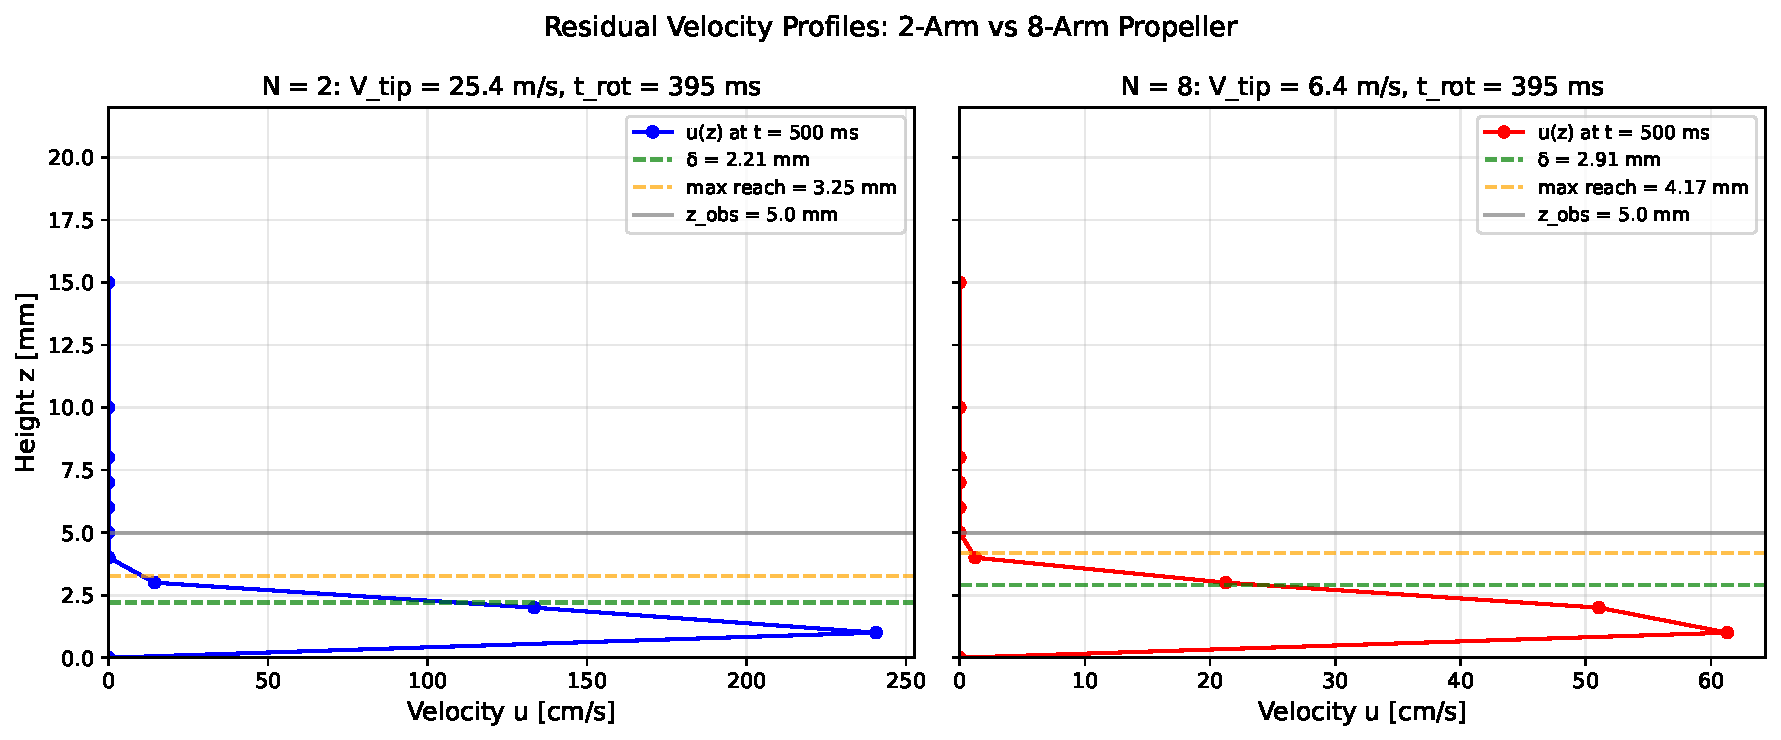
\includegraphics[width=\textwidth]{velocity_profiles_comparison.pdf}
\caption{Residual velocity profiles at $t_\mathrm{obs} = \SI{500}{ms}$ after
blade stops. Left: $n = 2$ ($V_\mathrm{tip} = \SI{25.4}{m/s}$). Right:
$n = 8$ ($V_\mathrm{tip} = \SI{6.4}{m/s}$). Green dashed line: BL thickness
$\delta$. Orange dashed line: maximum diffusion reach. Gray solid line:
observation height $z_\mathrm{obs} = \SI{5}{mm}$.}
\label{fig:profiles}
\end{figure}


% ══════════════════════════════════════════════════════════════════════════════
\section{Phase 2: Carrier Slide Results}
\label{sec:results_carrier}
% ══════════════════════════════════════════════════════════════════════════════

\begin{table}[H]
\centering
\caption{Carrier slide kinematics ($m_\mathrm{carrier} = \SI{0.25}{kg}$,
$F_\mathrm{act} = \SI{20}{N}$, $\Delta r = \SI{0.8}{m}$).}
\label{tab:carrier_kinematics}
\begin{tabular}{lcc}
\toprule
Quantity & Value & Units \\
\midrule
Acceleration $a = F/m$ & 80 & m/s$^2$ \\
Slide time $t_\mathrm{slide}$ & 200 & ms \\
Peak velocity $V_\mathrm{max}$ & 8.0 & m/s \\
\bottomrule
\end{tabular}
\end{table}

\begin{table}[H]
\centering
\caption{Carrier boundary layer and diffusion (same for $n = 2$ and $n = 8$).}
\label{tab:carrier_BL}
\begin{tabular}{lcc}
\toprule
Quantity & Value & Units \\
\midrule
Carrier Reynolds number Re$_L$ & $4.4 \times 10^6$ & --- \\
BL thickness $\delta_c$ & 2.78 & mm \\
Max reach & 4.0 & mm \\
Reach vs $z_\mathrm{obs}$ & $4.0 < 5.0$ & --- \\
\midrule
\textbf{Result: $u(z_\mathrm{obs}, t_\mathrm{obs})$} & \textbf{0} & m/s \\
\bottomrule
\end{tabular}
\end{table}

The carrier slide produces a boundary layer similar to the blade, but with
lower peak velocity. The maximum diffusion reach is still less than
$z_\mathrm{obs}$, confirming that the carrier slide does not contribute
residual velocity at the observation point.


% ══════════════════════════════════════════════════════════════════════════════
\section{Phase 3: Vertical Lift Results}
\label{sec:results_lift}
% ══════════════════════════════════════════════════════════════════════════════

\begin{table}[H]
\centering
\caption{Phase 3 kinematics ($z_\mathrm{lift} = \SI{5}{mm}$,
$t_\mathrm{lift} = \SI{1.0}{s}$, $t_\mathrm{wait} = \SI{0.5}{s}$).}
\label{tab:lift_kinematics}
\begin{tabular}{lcc}
\toprule
Quantity & Value & Units \\
\midrule
Lift height $z_\mathrm{lift}$ & 5.0 & mm \\
Lift duration $t_\mathrm{lift}$ & 1.0 & s \\
Lift acceleration $a_\mathrm{lift}$ & 0.020 & m/s$^2$ \\
Peak lift velocity $V_\mathrm{lift}$ & 10.0 & mm/s \\
Wait time $t_\mathrm{wait}$ & 0.5 & s \\
Quiescence cutoff $u_c$ & 0.1 & mm/s \\
\bottomrule
\end{tabular}
\end{table}

\begin{table}[H]
\centering
\caption{Phase 3 velocity profiles and quiescence heights.}
\label{tab:lift_profiles}
\begin{tabular}{lccc}
\toprule
Quantity & Formula & $n = 2$ & $n = 8$ \\
\midrule
\multicolumn{4}{l}{\textit{Profile 1: Blade BL diffusion}} \\
Evaluation time $t_\mathrm{eval}$ & $t_\mathrm{slide} + t_\mathrm{lift} + t_\mathrm{wait}$
  & \SI{1.7}{s} & \SI{1.7}{s} \\
BL thickness $\delta_1$ & (from Phase 1) & \SI{2.21}{mm} & \SI{2.91}{mm} \\
Decay time $t_\mathrm{decay}$ & $2\,t_e$ & \SI{3.5}{ms} & \SI{18}{ms} \\
Quiescence height $z_{q1}$ & (where $u < u_c$) & \SI{0.1}{mm} & \SI{2.9}{mm} \\
\midrule
\multicolumn{4}{l}{\textit{Profile 2: Carrier slide BL diffusion}} \\
Evaluation time $t_\mathrm{eval}$ & $t_\mathrm{lift} + t_\mathrm{wait}$
  & \SI{1.5}{s} & \SI{1.5}{s} \\
BL thickness $\delta_2$ & (from Phase 2) & \SI{2.78}{mm} & \SI{2.78}{mm} \\
Decay time $t_\mathrm{decay}$ & $2\,t_e$ & \SI{14}{ms} & \SI{14}{ms} \\
Quiescence height $z_{q2}$ & (where $u < u_c$) & \SI{2.8}{mm} & \SI{2.8}{mm} \\
\midrule
\multicolumn{4}{l}{\textit{Profile 3: Stokes layer from lift}} \\
Evaluation time $t_\mathrm{eval}$ & $t_\mathrm{wait}$
  & \SI{0.5}{s} & \SI{0.5}{s} \\
Stokes layer $\delta_3$ & $\sqrt{\nu\,t_\mathrm{lift}}$
  & \SI{0.54}{mm} & \SI{0.54}{mm} \\
Effective diffusion length $\delta_\mathrm{eff}$ & $\sqrt{\nu\,t_\mathrm{total}}$
  & \SI{0.66}{mm} & \SI{0.66}{mm} \\
Quiescence height $z_{q3}$ & (where $u < u_c$, in RF1)
  & \SI{7.5}{mm} & \SI{7.5}{mm} \\
\bottomrule
\end{tabular}
\end{table}

\paragraph{Key Observations.}
\begin{itemize}[nosep]
  \item \textbf{Profile 1} (blade BL): By the time of evaluation ($t = \SI{1.7}{s}$
    after rotation), the blade BL has essentially completely decayed for
    the $n = 2$ case (decay time is only \SI{3.5}{ms}). The $n = 8$ case
    has slightly longer decay (\SI{18}{ms}) but is still fully quiescent
    within $z_{q1} = \SI{2.9}{mm}$.
  \item \textbf{Profile 2} (carrier slide BL): Similarly decayed by evaluation
    time ($t = \SI{1.5}{s}$). The carrier BL parameters are identical for
    both $n = 2$ and $n = 8$ since the slide motion is the same.
  \item \textbf{Profile 3} (Stokes layer from lift): The vertical lift creates
    the dominant residual velocity. The erfc profile gives quiescence at
    $z_{q3} = \SI{7.5}{mm}$ (in RF1 coordinates).
  \item Since the plate surface is at $z = z_\mathrm{lift} = \SI{5}{mm}$,
    the quiescence height $z_{q3} = \SI{7.5}{mm}$ is \SI{2.5}{mm}
    above the plate surface.
\end{itemize}

\begin{figure}[H]
\centering
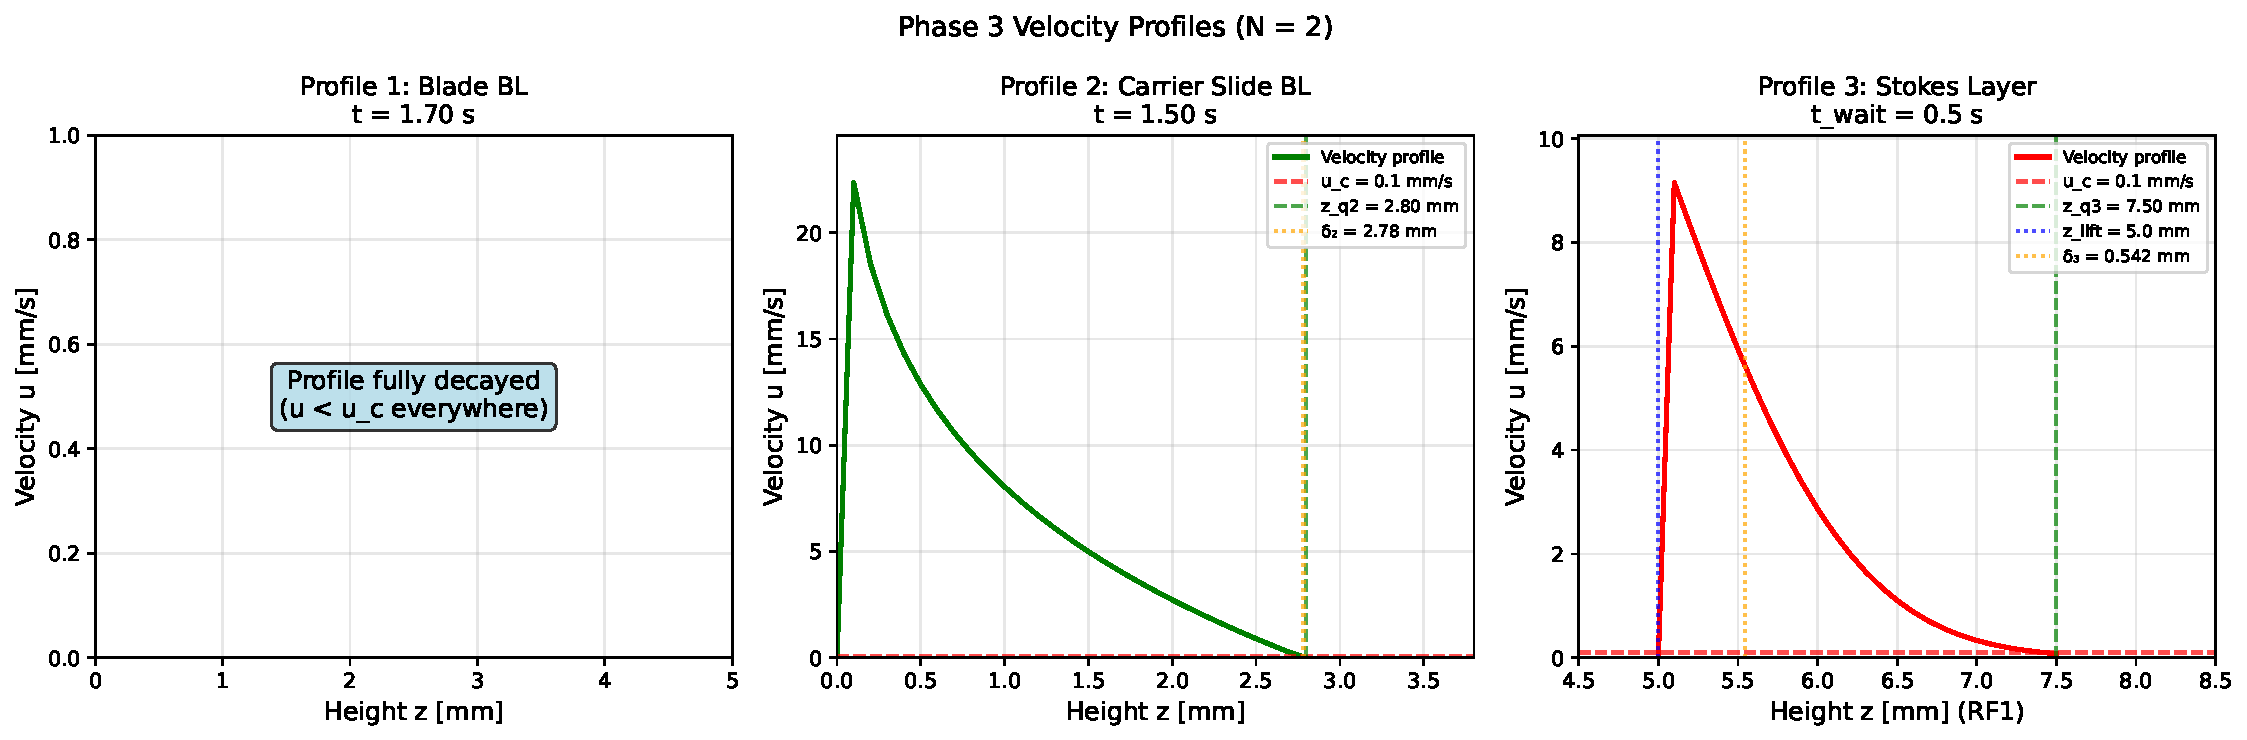
\includegraphics[width=\textwidth]{phase3_profiles_n2.pdf}
\caption{Phase 3 velocity profiles for $n = 2$. Left: Profile 1 (blade BL
diffusion, fully decayed). Center: Profile 2 (carrier slide BL diffusion).
Right: Profile 3 (Stokes layer from lift at $t_\mathrm{wait} = \SI{0.5}{s}$).
Red dashed line: quiescence cutoff $u_c = \SI{0.1}{mm/s}$. Green dashed
line: quiescence height $z_q$.}
\label{fig:phase3_n2}
\end{figure}

\begin{figure}[H]
\centering
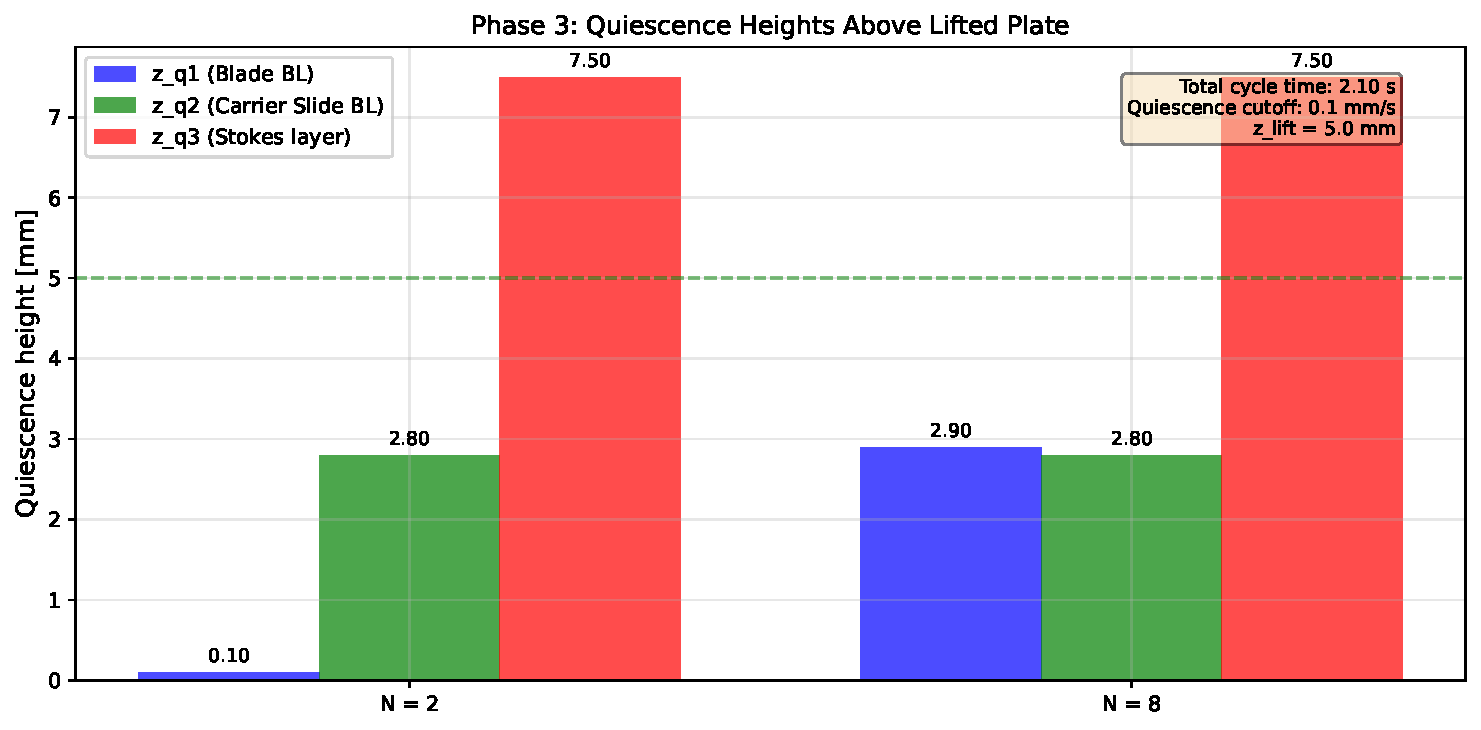
\includegraphics[width=\textwidth]{phase3_quiescence_comparison.pdf}
\caption{Comparison of quiescence heights for $n = 2$ and $n = 8$
configurations. $z_{q1}$ (blade BL) is very small for $n = 2$ due to fast
turbulence decay. $z_{q2}$ (carrier slide BL) is identical for both cases.
$z_{q3}$ (Stokes layer) is identical since lift parameters are the same.}
\label{fig:phase3_comparison}
\end{figure}


% ══════════════════════════════════════════════════════════════════════════════
\section{Mechanism 2: Bulk Swirl Results}
\label{sec:results_swirl}
% ══════════════════════════════════════════════════════════════════════════════

\begin{table}[H]
\centering
\caption{Bulk swirl and Ekman pumping parameters.}
\label{tab:swirl}
\begin{tabular}{lcc}
\toprule
Quantity & $n = 2$ & $n = 8$ \\
\midrule
Drag torque $\tau_\mathrm{drag}$ & \SI{31.3}{N\cdot m} & \SI{10.3}{N\cdot m} \\
Angular impulse $J$ & \SI{15.6}{N\cdot m\cdot s} & \SI{5.2}{N\cdot m\cdot s} \\
\midrule
Mol.\ diffusion time $t_\mathrm{visc}$ & \SI{25}{s} & \SI{13}{s} \\
Ratio $t_\mathrm{visc}/t_\mathrm{obs}$ & 50 & 26 \\
\midrule
Ekman thickness (mol.) $\delta_E$ & \SI{0.22}{mm} & \SI{0.43}{mm} \\
Ekman velocity (mol.) $w_E$ & \SI{1.4}{mm/s} & \SI{0.68}{mm/s} \\
Ekman thickness (turb.) $\delta_E$ & \SI{4.1}{mm} & \SI{4.7}{mm} \\
Ekman velocity (turb.) $w_E$ & \SI{2.6}{cm/s} & \SI{0.74}{cm/s} \\
Turb.\ vertical reach & \SI{0.12}{mm} & \SI{0.18}{mm} \\
\midrule
Ekman spin-up (mol.) & \SI{736}{s} & \SI{1472}{s} \\
Ekman spin-up (turb.) & \SI{39}{s} & \SI{136}{s} \\
\midrule
\textbf{Result: $u(z_\mathrm{obs}, t_\mathrm{obs})$} & \textbf{0} & \textbf{0} \\
\bottomrule
\end{tabular}
\end{table}

Momentum stays confined to the blade plane. No transport mechanism
operates within $t_\mathrm{obs} = \SI{0.5}{s}$.


% ══════════════════════════════════════════════════════════════════════════════
\section{Mechanisms 3--6 Results}
\label{sec:results_other}
% ══════════════════════════════════════════════════════════════════════════════

\begin{table}[H]
\centering
\caption{Displacement flow and pressure pulse parameters.}
\label{tab:potential}
\begin{tabular}{lcc}
\toprule
Quantity & $n = 2$ & $n = 8$ \\
\midrule
Displacement velocity $w_\mathrm{disp}$ (during sweep) & \SI{15.8}{m/s} & \SI{4.0}{m/s} \\
Acoustic clearing time $t_\mathrm{acoustic}$ & \SI{9.0}{ms} & \SI{9.0}{ms} \\
Ratio $t_\mathrm{obs}/t_\mathrm{acoustic}$ & 56 & 56 \\
\textbf{Result: potential flow} & \textbf{0} & \textbf{0} \\
\midrule
Pressure perturbation $\Delta p$ & \SI{31892}{Pa} & \SI{1993}{Pa} \\
Fractional $\Delta p / P$ & 2.1\% & 0.13\% \\
Induced velocity $\Delta u$ & \SI{2.3}{m/s} & \SI{0.14}{m/s} \\
\textbf{Result: pressure pulse} & \textbf{0} & \textbf{0} \\
\midrule
Centrifugal acceleration $a_\mathrm{cent}$ & \SI{63}{m/s^2} & \SI{3.9}{m/s^2} \\
Tip gap traversal time & \SI{0.04}{s} & \SI{0.16}{s} \\
\textbf{Result: secondary flows} & \textbf{0} & \textbf{0} \\
\midrule
Shedding frequency (bluff ref.) & \SI{220}{Hz} & \SI{55}{Hz} \\
\textbf{Result: vortex shedding} & \textbf{0} & \textbf{0} \\
\bottomrule
\end{tabular}
\end{table}


% ══════════════════════════════════════════════════════════════════════════════
\section{Comparison: 2-Arm vs 8-Arm}
\label{sec:comparison}
% ══════════════════════════════════════════════════════════════════════════════

\begin{table}[H]
\centering
\caption{Comparison of key parameters between 2-arm and 8-arm configurations.}
\label{tab:comparison}
\begin{tabular}{lccc}
\toprule
Quantity & $n = 2$ & $n = 8$ & Ratio (2/8) \\
\midrule
\textbf{Phase 1: Blade Rotation} & & & \\
Moment of inertia $I$ & \SI{0.75}{kg\cdot m^2} & \SI{2.99}{kg\cdot m^2} & 0.25 \\
Sweep angle $\theta$ & 180° & 45° & 4 \\
Rotation time $t_\mathrm{rot}$ & \SI{396}{ms} & \SI{396}{ms} & 1 \\
Peak tip velocity $V_\mathrm{tip}$ & \SI{25.4}{m/s} & \SI{6.4}{m/s} & 4 \\
\midrule
\textbf{Flow Regime} & & & \\
Reynolds number $\mathrm{Re}_c$ & $1.38 \times 10^7$ & $3.46 \times 10^6$ & 4 \\
Mach number Ma & 0.143 & 0.036 & 4 \\
\midrule
\textbf{Boundary Layer} & & & \\
BL thickness $\delta$ & \SI{2.21}{mm} & \SI{2.91}{mm} & 0.76 \\
Gap to observation & \SI{2.8}{mm} & \SI{2.1}{mm} & 1.3 \\
\midrule
\textbf{Diffusion} & & & \\
Eddy decay time $2t_e$ & \SI{3.5}{ms} & \SI{18}{ms} & 0.19 \\
Max diffusion reach & \SI{3.3}{mm} & \SI{4.2}{mm} & 0.78 \\
\midrule
\textbf{Phase 2: Carrier Slide} & & & \\
Slide time $t_\mathrm{slide}$ & \SI{200}{ms} & \SI{200}{ms} & 1 \\
Peak velocity $V_\mathrm{max}$ & \SI{8.0}{m/s} & \SI{8.0}{m/s} & 1 \\
Carrier BL thickness $\delta_c$ & \SI{2.78}{mm} & \SI{2.78}{mm} & 1 \\
Carrier max reach & \SI{4.0}{mm} & \SI{4.0}{mm} & 1 \\
\midrule
\textbf{Phase 3: Vertical Lift} & & & \\
Lift time $t_\mathrm{lift}$ & \SI{1.0}{s} & \SI{1.0}{s} & 1 \\
Lift height $z_\mathrm{lift}$ & \SI{5.0}{mm} & \SI{5.0}{mm} & 1 \\
Peak lift velocity $V_\mathrm{lift}$ & \SI{10}{mm/s} & \SI{10}{mm/s} & 1 \\
Stokes layer $\delta_3$ & \SI{0.54}{mm} & \SI{0.54}{mm} & 1 \\
Wait time $t_\mathrm{wait}$ & \SI{0.5}{s} & \SI{0.5}{s} & 1 \\
\midrule
\textbf{Total Cycle Time} & \SI{2.10}{s} & \SI{2.10}{s} & 1 \\
\midrule
\textbf{Residual Velocity (Phase 1)} & $3.2 \times 10^{-7}$ m/s & $3.3 \times 10^{-5}$ m/s & --- \\
\textbf{Residual Velocity (Phase 2)} & \textbf{0} & \textbf{0} & --- \\
\textbf{Quiescence height $z_{q1}$} (blade BL) & \SI{0.1}{mm} & \SI{2.9}{mm} & --- \\
\textbf{Quiescence height $z_{q2}$} (carrier BL) & \SI{2.8}{mm} & \SI{2.8}{mm} & 1 \\
\textbf{Quiescence height $z_{q3}$} (Stokes) & \SI{7.5}{mm} & \SI{7.5}{mm} & 1 \\
\bottomrule
\end{tabular}
\end{table}


% ══════════════════════════════════════════════════════════════════════════════
\section{Summary}
\label{sec:summary}
% ══════════════════════════════════════════════════════════════════════════════

\begin{table}[H]
\centering
\caption{Summary of all mechanisms for residual velocity.}
\label{tab:summary}
\begin{tabular}{lccc}
\toprule
Mechanism & Timescale & $n = 2$ result & $n = 8$ result \\
\midrule
\multicolumn{4}{l}{\textit{Phase 1: Blade rotation}} \\
1. Eddy diffusion    & $2t_e \sim 4$--18 ms  & $3.2 \times 10^{-7}$ m/s & $3.3 \times 10^{-5}$ m/s \\
2. Bulk swirl        & $t_\mathrm{visc} \sim 13$--25 s & 0 & 0 \\
3. Potential flow    & $t_\mathrm{acoustic} \approx 9$ ms & 0 & 0 \\
4. Pressure pulse    & $t_\mathrm{decel} \sim 10$ ms & 0 & 0 \\
5. Secondary flows   & $t_\mathrm{Ekman} \sim 39$--136 s & 0 & 0 \\
6. Vortex shedding   & N/A (confined) & 0 & 0 \\
\midrule
\multicolumn{4}{l}{\textit{Phase 2: Carrier slide}} \\
7. Carrier eddy diff. & max reach $< z_\mathrm{obs}$ & 0 & 0 \\
\midrule
\multicolumn{4}{l}{\textit{Phase 3: Vertical lift (three profiles)}} \\
8. Blade BL ($z_{q1}$) & eval at $t = \SI{1.7}{s}$ & \SI{0.1}{mm} & \SI{2.9}{mm} \\
9. Carrier BL ($z_{q2}$) & eval at $t = \SI{1.5}{s}$ & \SI{2.8}{mm} & \SI{2.8}{mm} \\
10. Stokes layer ($z_{q3}$) & eval at $t_\mathrm{wait}$ & \SI{7.5}{mm} & \SI{7.5}{mm} \\
\bottomrule
\end{tabular}
\end{table}

\subsection{Conclusion}

For both the 2-arm and 8-arm propeller configurations, the gas above
the lifted carrier plate becomes \textbf{quiescent} (velocity $< \SI{0.1}{mm/s}$)
within the total cycle time of approximately \SI{2.1}{s}.

The complete motion sequence is:
\begin{enumerate}[nosep]
  \item \textbf{Phase 1}: Blade rotation ($t_\mathrm{rot} = \SI{396}{ms}$)
  \item \textbf{Phase 2}: Carrier slide ($t_\mathrm{slide} = \SI{200}{ms}$)
  \item \textbf{Phase 3}: Vertical lift ($t_\mathrm{lift} = \SI{1.0}{s}$)
  \item \textbf{Wait period}: ($t_\mathrm{wait} = \SI{0.5}{s}$)
  \item \textbf{Total cycle}: $t_\mathrm{total} \approx \SI{2.1}{s}$
\end{enumerate}

\paragraph{Phase 3 Analysis.}
After the vertical lift, three velocity profiles determine the quiescence:
\begin{itemize}[nosep]
  \item \textbf{Profile 1} (blade BL): By the time the lift completes and
    wait period ends ($\sim\SI{1.7}{s}$ after rotation), the blade boundary
    layer has fully decayed. For $n = 2$, $z_{q1} = \SI{0.1}{mm}$ (essentially
    zero). For $n = 8$, $z_{q1} = \SI{2.9}{mm}$.
  \item \textbf{Profile 2} (carrier slide BL): Evaluated at $t = \SI{1.5}{s}$
    after the slide stopped. The carrier BL also decays rapidly, giving
    $z_{q2} = \SI{2.8}{mm}$ for both configurations (since the slide
    parameters are identical).
  \item \textbf{Profile 3} (Stokes layer): The vertical lift creates a thin
    Stokes layer ($\delta_3 = \SI{0.54}{mm}$). After $t_\mathrm{wait} = \SI{0.5}{s}$,
    quiescence is reached at $z_{q3} = \SI{7.5}{mm}$ in RF1 coordinates.
    Since the plate surface is at $z = \SI{5}{mm}$, the quiescent region
    begins \SI{2.5}{mm} above the plate.
\end{itemize}

\paragraph{Key Results.}
The 8-arm propeller has 4$\times$ lower peak velocity than the 2-arm,
resulting in:
\begin{itemize}[nosep]
  \item 4$\times$ lower Reynolds number (still fully turbulent)
  \item 4$\times$ lower Mach number (both incompressible)
  \item Thicker BL but slower turbulent decay
  \item Similar total diffusion reach (both insufficient to reach $z_\mathrm{obs}$)
\end{itemize}

The fundamental reason for effective quiescence is that:
\begin{enumerate}[nosep]
  \item The NACA\,0012 at zero angle of attack produces no lift, so all
    aerodynamic effects are confined to the thin drag wake within
    $\delta \approx 2$--$3$ mm of the surface.
  \item The dense xenon gas ($\rho \approx \SI{79}{kg/m^3}$) has extremely
    small kinematic viscosity ($\nu \approx \SI{3e-7}{m^2/s}$), making all
    diffusion timescales very long.
  \item Turbulent eddies are small ($\sim\delta$) and decay rapidly
    ($\sim$\SI{3}{ms}--\SI{18}{ms}) once the motion stops. By the time
    of evaluation ($\sim$\SI{1.5}{s}--\SI{1.7}{s}), both blade and carrier
    boundary layers have fully decayed.
  \item The vertical lift velocity ($V_\mathrm{lift} = \SI{10}{mm/s}$) is
    very low, creating only a thin Stokes layer ($\delta_3 \approx \SI{0.5}{mm}$).
  \item The dominant residual flow is Profile 3 (Stokes layer), which gives
    quiescence at $z_{q3} = \SI{7.5}{mm}$, just \SI{2.5}{mm} above the
    lifted plate surface.
\end{enumerate}

\begin{figure}[H]
\centering
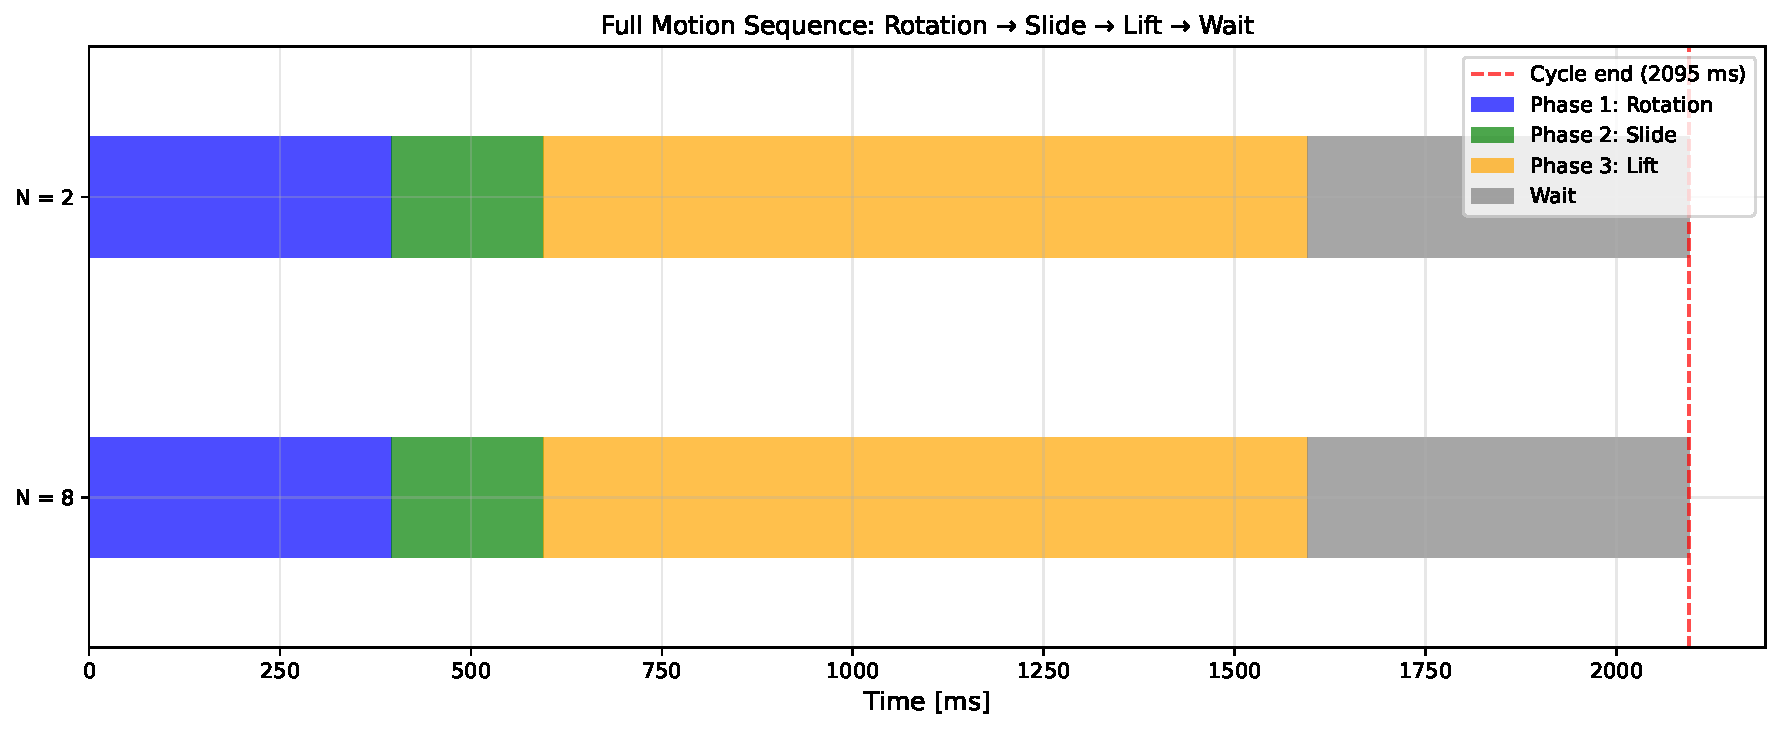
\includegraphics[width=\textwidth]{full_timeline.pdf}
\caption{Complete motion timeline showing all three phases: blade rotation
(Phase 1, blue), carrier slide (Phase 2, green), vertical lift (Phase 3,
orange), and wait period (gray). The total cycle time is approximately
\SI{2.1}{s} for both configurations.}
\label{fig:timeline}
\end{figure}

\begin{figure}[H]
\centering
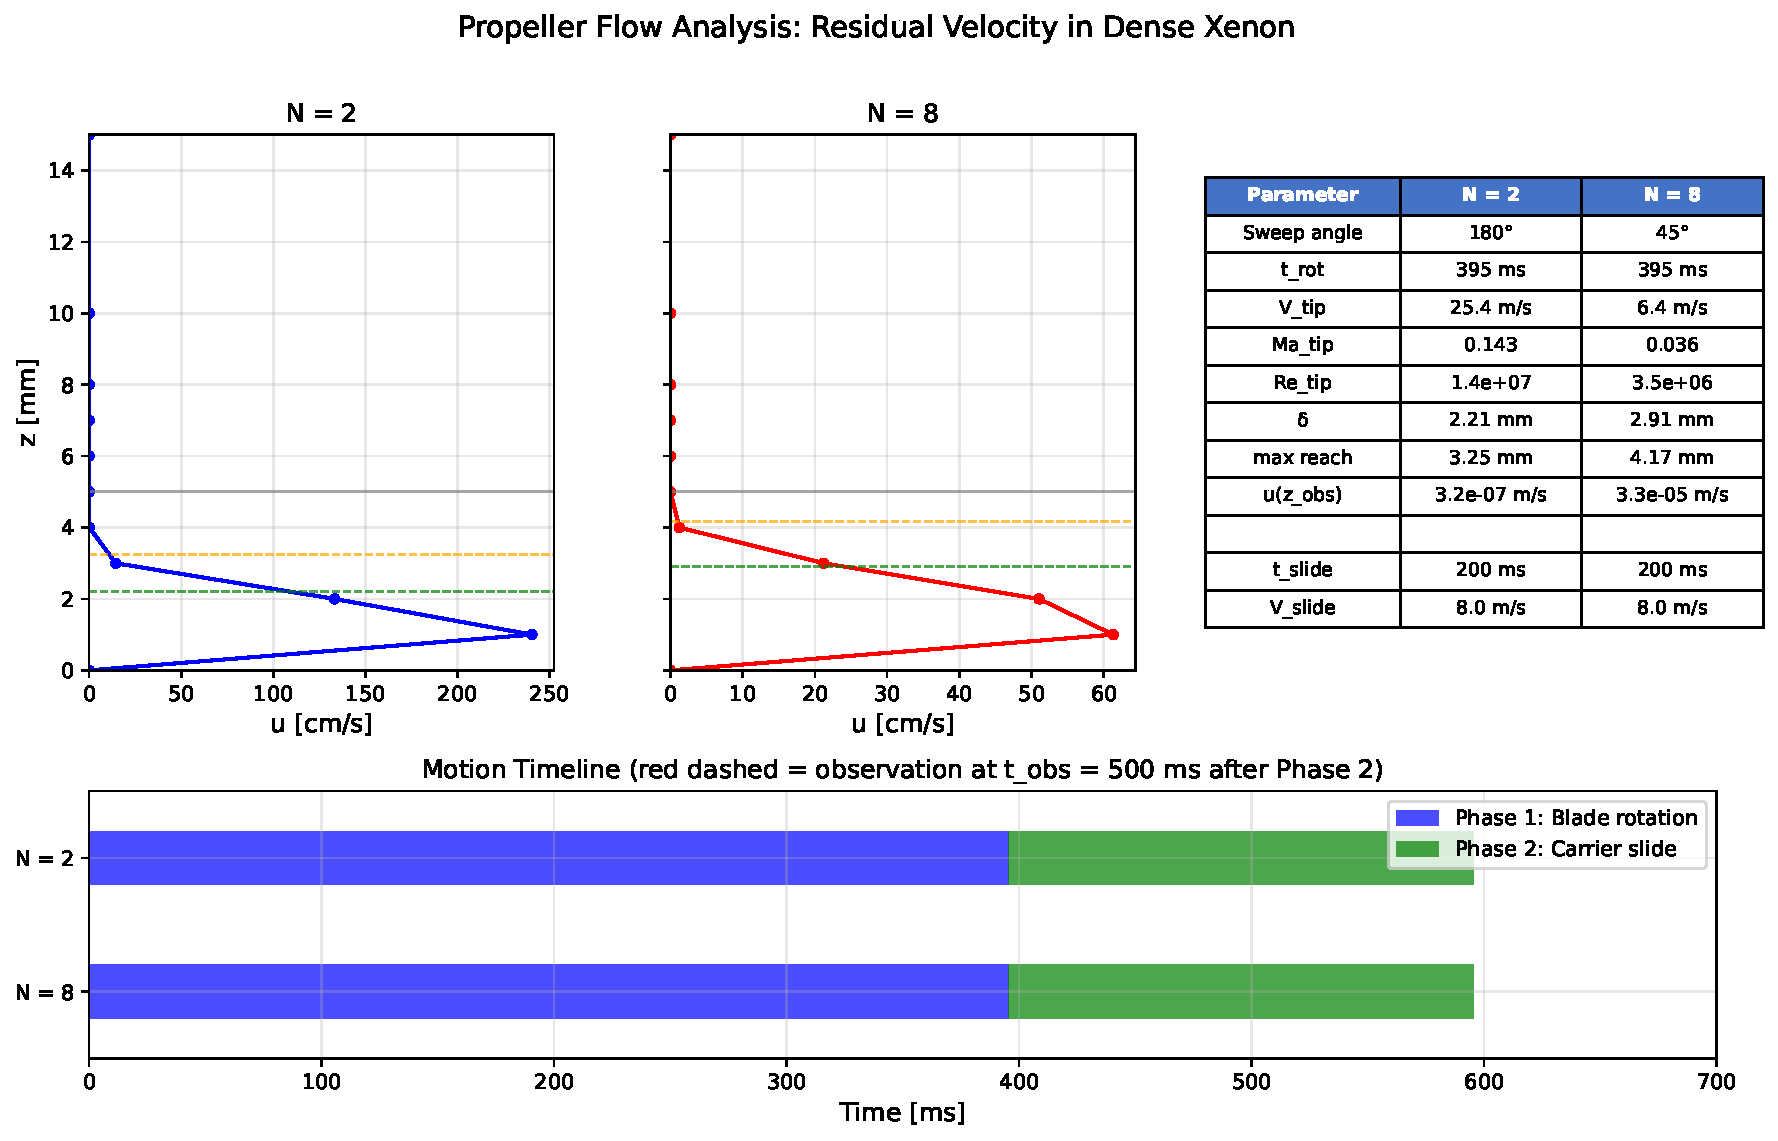
\includegraphics[width=\textwidth]{propeller_analysis_summary.pdf}
\caption{Summary of Phase 1 and 2 analysis showing velocity profiles,
key parameters comparison, and motion timeline for $n = 2$ and $n = 8$
configurations.}
\label{fig:summary}
\end{figure}

\end{document}
